% !TEX root =  ./main.tex

\subsection{GT and GROOVE}\label{sec:GTS}

Graph Transformation (or Graph Rewriting) is well-established rule-based formalism, the core of which is to specify precisely how graphs may evolve. Each rule embodies a particular change, which can be applied to a given graph (in the simplest form consisting of nodes and binary edges) by establishing where in that graph the preconditions of the rule are met, and then adding and deleting nodes and edges as prescribed.

In this paper, we use the so-called \emph{algebraic approach} to graph transformation (see \cite{DBLP:series/eatcs/EhrigEPT06} for a formal exposition and \cite{DBLP:books/sp/HeckelT20} for applications in the context of software engineering); moreover, we rely on the particular flavour implemented in the tool GROOVE \cite{DBLP:journals/sttt/GhamarianMRZZ12,GROOVE}. Some of the relevant features of the approach and the tool are highlighted below.
%\todo{RB: the previous itemized list has been just commented in the source .tex, not deleted}
%
%\begin{itemize}
%\item Graphs are \emph{directed} and \emph{typed}, meaning that nodes and edges have labels, and edges have a direction (going from their \emph{source} to their \emph{target}). Besides binary edges, nodes can also have \emph{flags} (which are actually self-loops that act as additional, optional labels on nodes) and \emph{attributes} (which are actually binary edges whose target node is a data value, e.g., an integer or string).
%
%\item Rules consist of a left hand side (LHS) and right hand side (RHS). Rule applicability is established by \emph{matching} the LHS to the graph in question, and where a match exists, removing nodes and edges that are in the LHS but not in the RHS, and vice versa, adding nodes and edges that are in the RHS but not in the LHS.
%
%\item \GROOVE graphs are \emph{simple} (rather than \emph{multi-sorted}), meaning that there is at most one edge of a given type between any two nodes, and similarly, at most one flag of a given type on any node. If an edge or flag is added where one exists already, this does not change the graph.
%
%\item \GROOVE rules may be \emph{quantified}, meaning that they can simultaneously be applied to multiple places in the same graph. An example is shown in \Cref{fig:context} below.
%
%\item A graph transformation \emph{system} is a set of rules. In the simplest case, every rule can be applied to a graph at hand, giving rise to a modified graph to which every rule can be applied again, and so forth. However, \GROOVE allows rule application to be restricted by an external \emph{control program} that can specify in what order rules may be applied.
%
%\item The core functionality of \GROOVE is to explore the set of reachable graphs, given a graph transformation system (with or without control program) and an initial graph. With this as the basis, there are built-in strategies for searching and model checking.
%\end{itemize}
%

\textbf{Graphs} are \emph{simple} and \emph{typed}, meaning that there is at most one edge of a given type between any two nodes and that all nodes and edges are labelled through a morphism to a given (fixed) \emph{type graph}. Edges are \emph{directed} (going from their \emph{source} to their \emph{target}). Besides binary edges, nodes can also have \emph{flags} (which are actually self-loops that act as additional, optional labels on nodes) and \emph{attributes} (which are actually binary edges whose target node is a data value, e.g., an integer or a string).

\textbf{Rules}, in their simplest form, consist of a left hand side (LHS) and right hand side (RHS). Rule applicability is established by \emph{matching} the LHS to the graph in question, and where a match exists, removing nodes and edges that are in the LHS but not in the RHS, and vice versa, adding nodes and edges that are in the RHS but not in the LHS. In addition, however, \GROOVE supports \emph{quantified} rules, which can simultaneously be applied to multiple places in the same graph. An example is shown in \Cref{fig:context} below.

\textbf{Evolution} of a graph is defined on the basis of a graph transformation \emph{system}, which is a set of rules applied to a graph at hand, giving rise to a modified graph to which every rule can be applied again, and so forth. On top of this, \GROOVE allows for \emph{control programs} that can specify in what order rules may be applied. By exploring the potential evolution of a graph in all ways allowed by the control program, \GROOVE constructs the \emph{state space} of the graph transformation system, in the form of a \emph{labelled transition system} consisting of all reachable graphs and the rule applications between them.

\textbf{Analysis} consists of the exploration of the state space for a given initial graph, rule system and (optional) control program. The exploration can be tuned by built-in strategies for searching and model checking.
%\todo{RB: slightly rearranged}
%The core functionality of \GROOVE is to explore the set of reachable graphs, given a graph transformation system (with or without control program) and an initial graph. With this as the basis, there are built-in strategies for searching and model checking.

\medskip\noindent
The power of graph transformation lies in its generality: many systems naturally lend themselves to be modelled as graphs, and algebraic rules --- especially quantified ones --- provide a rich framework to specify their evolution. This is in fact our motivation for using it the current paper: reaction systems can straightforwardly be interpreted as graphs. \Cref{fig:core-type} shows the core types for the relevant concepts of that interpretation. (The colours just support the visualisation and have no semantics of their own.)

\begin{figure}
\centering
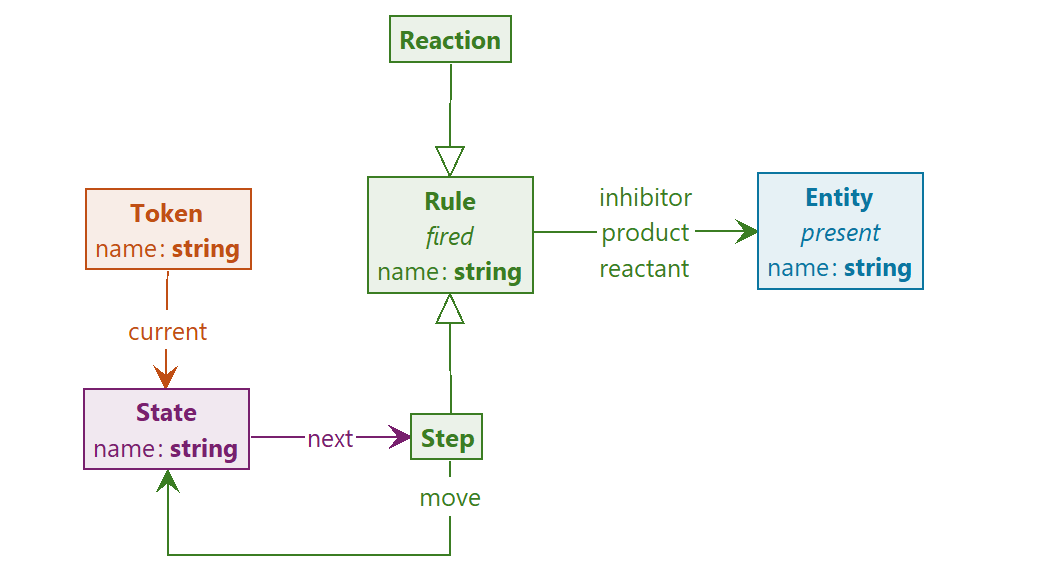
\includegraphics[scale=.2]{figs/core-type}
\caption{Core type graph for reaction systems}
\label{fig:core-type}
\end{figure}
%
Note especially the (abstract) supertype \Rule with subtypes \Reaction and \Step: the former is the type for the elements of $A$ in a Reaction System ${\cal A}=(S,A)$, whereas the latter is used to represent triples $(R,I,P)$ in a context RS process (\Cref{def:LTSforRS}). The set $S$ is represented by nodes of type \Entity; for a given \Rule, the subsets $R$, $I$, and $P$ of $S$ are those \Entity{}s to which there is an outgoing edge labelled \reactant, \inhibitor or \product. The flag \present is used to label the entities occurring in a state $W$. Finally, the structure of (guarded) context processes is captured by \State entities, with \nextt-edges to the \Step{}s that can be nondeterministally chosen; the subsequent process after such a \Step is determined by its outgoing \move-edge. \Token nodes are used to model which \State{}s are currently active.

